\phantomsection
\chapter{Local Binary Patterns}
\label{chap:lbp}

\noindent Some feature extractions are widely used and studied as the Principal Component Analysis (PCA) and the Linear Discriminant Analysis (LDA) to characterize and describe the face. They in fact describe the whole face. But these method are not efficient when the lightning changes or when the pose of the head changes. This is quite a challenge for these method. That is why some researchers turned to local descriptors. These local descriptors describe the face by characterize the parts of the face in function of their importance. The Local Binary Pattern (LBP) feature extraction is a local descriptor and it is widely used \cite{AHO06}.
\newline

\noindent The LBP operator is one of the best performing texture descriptor. It has been introduced in 1996 by Ojala et al. \cite{OJA96}. It is also one of the most widely used. This operator has a lot of advantages. One of its main advantages is that this operator is highly discriminative. The other advantages are its invariance to gray-level changes and its computation efficiency. Its computation efficiency is suitable for image analysis but it may not be efficient enough for real-time analysis \cite{AHO06}.
\newline

\noindent LBP is known to be a great operator for texture description but why is it used for face description? Because faces can be seen as a composition of micro-patterns. And describing micro-patterns is what the LBP operator does \cite{AHO06}.
\newline

\phantomsection
\section{Overview}

\vspace{\baselineskip}
\noindent Globally, a gray-scale image of a face is divided into small regions. LBP histograms are extracted from each of those small regions. Then these histogram are concatenated into a single feature vector \cite{JUL07}.
\newline

\noindent The LBP operator works with one central pixel and its eight neighbor pixels. It is basically a comparison with a threshold between the central pixel and the neighbor pixels. The intensity value of the central pixel sets the threshold. Then for each neighbor pixels, the same method is applied. If a neighbor pixel has a value superior to the one of the central pixel or equal to, a 1 is assigned to this pixel. If the pixel value of the neighbor pixel is inferior to the one of the central pixel, then a 0 is assigned to this pixel. Then, when all the neighbor pixels are done, a LBP code for the central pixel can be obtained by concatenating all the values of the eight neighbor pixels into a binary code. And for a better comprehension for the human, this code can also be transformed from a binary code to a decimal one. The figure~\ref{lbp_basic_operator} shows an example of the LBP process for a central pixel and its eight neighbor pixels \cite{JUL07}.
\newline

\begin{figure}[!h]
\begin{center}
\noindent 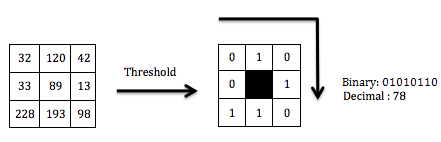
\includegraphics[scale=0.5]{figures/lbp_basic_operator} 
\newline
\caption{The LBP operator}
\label{lbp_basic_operator}
\end{center} 
\end{figure}

\noindent The LBP operator works with one central pixel and its eight neighbor pixels. It is basically a comparison with a threshold between the central pixel and the neighbor pixels. The intensity value of the central pixel sets the threshold. Then for each neighbor pixels, the same method is applied. If a neighbor pixel has a value superior to the one of the central pixel or equal to, a 1 is assigned to this pixel. If the pixel value of the neighbor pixel is inferior to the one of the central pixel, then a 0 is assigned to this pixel. Then, when all the neighbor pixels are done, a LBP code for the central pixel can be obtained by concatenating all the values of the eight neighbor pixels into a binary code. And for a better comprehension for the human, this code can also be transformed from a binary code to a decimal one. The figure~\ref{lbp_basic_operator} shows an example of the LBP process for a central pixel and its eight neighbor pixels \cite{JUL07}. The figure~\ref{lbp_basic_operator_example} shows an example of the LBP operator applied on a facial image from the JAFFE database \cite{LIU11}.
\newline

\begin{figure}[!h]
\begin{center}
\noindent 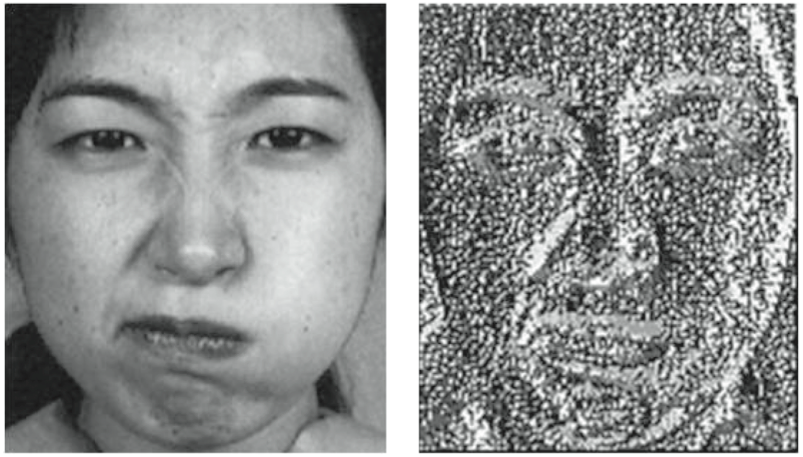
\includegraphics[scale=0.5]{figures/lbp_basic_operator_example} 
\newline
\caption{Example of the LBP operator applied on a facial image from the JAFFE database}
\label{lbp_basic_operator_example}
\end{center} 
\end{figure}

\phantomsection
\section{Improvements}

\phantomsection
\subsection{Circular LBP}

\vspace{\baselineskip}
\noindent In order to be able to use the LBP operator at different scales, a new form of the operator was used. This new form is the "Circular LBP Operator". This way, the operator can be extended to other neighborhoods than only eight pixels; it can be extended to neighborhood of various sizes \cite{GAN08}.
\newline

\noindent This operator still compares the intensity value of the central pixel with the one of its neighbors but the neighbors pixels are now calculating by a circle as follows \cite{GAN08}:

\begin{itemize}
  \item P represents the number of sampling points (neighbor pixels)
  \item C represents the central pixel and has the coordinates $ (x_c,y_c) $
  \item R represents the distance between each of the neighbor pixels and the central pixel
\end{itemize}

\noindent To find the coordinates of each P neighbor pixel, the formula are the following \cite{JUL07}:
\newline

\begin{equation}
   x = x_c + R\cos(2\pi n/P)
\end{equation}

\begin{equation}
   y = y_c + R\sin(2\pi n/P)
\end{equation}

\vspace{\baselineskip}
\noindent The figure~\ref{lbp_circular_operator} shows the circular LBP operator with a different number of neighbor pixels P and with various sizes \cite{JUL07}. For the circular LBP operator, the following notation is used: $ (P,R) $ and for a pixel p, the following notation is used: $ LBP_{P,R}(p) $ \cite{GAN08}.
\newline

\begin{figure}[!h]
\begin{center}
\noindent 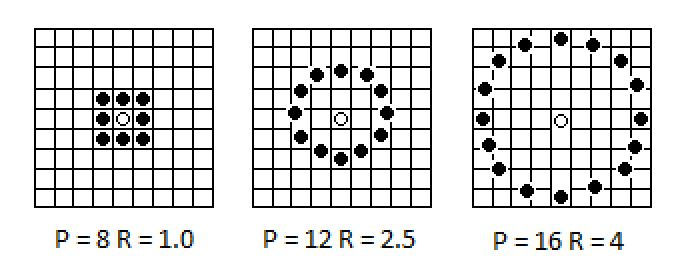
\includegraphics[scale=0.5]{figures/lbp_circular_operator} 
\newline
\caption{The circular LBP operator with different radius R and different number of neighbor pixels P}
\label{lbp_circular_operator}
\end{center} 
\end{figure}

\noindent Most of the time, when a circular LBP operator is used, the coordinates of the neighbor pixels (calculated with the formula given above) may not fall exactly on a pixel. In this case, using a bilinear interpolations of the neighbor pixel intensity values is recommended for the comparison. For example, the circular operator with $ P = 8 $ and $ R = 1.0 $ looks like the basic LBP operator; the only difference is that for the calculation, in case of the neighbor pixels do not fall right into single pixels, these pixel has to be interpolated first \cite{GAN08}.
\newline

\noindent What is resulting of the LBP operation is the texture. The formula of the texture is the following \cite{GAN08}:
\newline

\begin{equation}
   T = t(I_C, I_0, I_1, ..., I_{P-1})
\end{equation}

\vspace{\baselineskip}
\noindent With $ I_C $, the intensity value of the central pixel, $ I_p $ for $ p = 0, 1, ..., P $, the intensity values of the P neighbor pixels, with $ T $, the texture in the local neighborhood of $ C $ \cite{GAN08}.
\newline

\noindent But this texture can also be calculated in an other way. It consists in subtracting the central pixel intensity value from the pixel values of the computed neighborhood values. This way, the texture $ T $ is the combination of the differences between the intensity values of the neighbor pixels and the central pixel, and of the intensity value of the central pixel $ I_C $. The formula resulting is the following \cite{GAN08}:
\newline

\begin{equation}
   T = t(I_C, I_0 - I_C, I_1 - I_C, ..., I_{P-1} - I_C)
\end{equation}

\vspace{\baselineskip}
\noindent Based on the work of Ojala et al. \cite{OJA96}, $ t(I_C) $ describes the overall luminance of an image. The overall luminance is not related to the local texture of the image. And by consequent, relevant information for texture analysis are not provided. Even after dropping this element from the formula above, the texture description still contained the most of the texture information with the following formula \cite{GAN08}:
\newline

\begin{equation}
   T = t(I_0 - I_C, I_1 - I_C, ..., I_{P-1} - I_C)
\end{equation}

\vspace{\baselineskip}
\noindent The above formula makes the texture description invariant against shifts in the intensity values. But against scaling of the intensity values, the texture description is not invariant. To obtain a texture description invariant to these scalings, only the signs of the differences are taken into account (and not the difference in itself). The new formula is as follows \cite{GAN08}:
\newline

\begin{equation}
   T = t(s(I_0 - I_C), s(I_1 - I_C), ..., s(I_{P-1} - I_C))
\end{equation}

\noindent where,
\newline

\begin{equation}
s(x) = \left\{
    \begin{array}{ll}
        1 & \mbox{if } x\geq0 \\
        0 & \mbox{if } x < 0
    \end{array}
\right.
\end{equation}

\vspace{\baselineskip}
\noindent For the pixels with an intensity value superior or equal to the one of the central pixel, the sign assigned would be 1. For the pixels with an intensity value inferior to the one of the central pixel, the sign assigned would be 0 \cite{GAN08}.
\newline

\noindent The last step is to assign a binomial weight to each sign, for the LBP operation.These weights are summed and it produces for the central pixel $ C $ of coordinates $ (x_C,y_C) $, the LBP code. The formula is as follows \cite{GAN08}:
\newline

\begin{equation}
   LBP_{P,R}(x_C,y_C) = \sum_{p = 0}^{P-1} s(I_p - I_C)2^p
\end{equation}

\vspace{\baselineskip}
\noindent The use of the formula above to calculate LBP produce a large number of patterns and it does not help to reduce the size of data. That is why Uniform Local Binary Pattern are used; this way, LBP are used in an efficient way for image processing \cite{GAN08}. This kind of LBP will be explained in the subsection below.
\newline

\phantomsection
\subsection{Uniform LBP}

\vspace{\baselineskip}
\noindent A Local Binary Pattern can be called uniform only if it contains 2 or less bitwise transitions. A bitwise transitions can be a transition from 0 to 1 or the opposite: from 1 to 0 \cite{GAN08}. 
\newline

\noindent In fact, there can be only 2 or 0 bitwise transitions for a uniform LBP. Indeed, the LBP is circular so there cannot be only 1 bitwise transition. If at a moment on the circle, one pixel is at 1 and then after two pixel for example, there is a pixel at 0, this is one bitwise transition. But then, going on on the circle, there will be inevitably another bitwise transition from 0 to 1 to go back at the pixel with the value of 1 \cite{GAN08}.
\newline

\noindent If a pattern contains 0 bitwise transition, it means that it is composed only of 0s or of 1s \cite{GAN08}.
\newline

\noindent For a uniform LBP with a bit-length of 8 bits, containing 2 bitwise transitions, with P numbers of neighbor pixels, there are $ P(P - 1) $ possible combinations. So there are $ 8(8 - 1) + 2 =58 $ possible patterns ("$ + 2 $" is for the 2 patterns with 0 bitwise transition; the patterns with all 1s or all 0s). The uniform LBP has the following notation: \[ LBP_{P,R}^{u^2} \] with P numbers of neighbor pixels and R, the value of the radius \cite{GAN08}.
\newline

\noindent There are 2 main advantages coming along with the uniform LBP. The first one is the reduction in range of possible pattern that the uniform LBP allows. With the uniform LBP operator, there are 58 possible combinations as seen above. With the basic LBP operator, for the same bit-length, there are $ 2^8 = 256 $ possible combinations. More than four times more possible combinations \cite{GAN08}.
\newline

\noindent The second advantages is that even though there is a reduction of dimensionality thanks to the uniform LBP, the patterns are still discriminative between various structural features. These structural features still detected by the uniform LBP are the spot, the spot/flat, the line end, the edge and the corner. These features are shown in the figure~\ref{lbp_structural_features}  \cite{GAN08}.
\newline

\begin{figure}[!h]
\begin{center}
\noindent 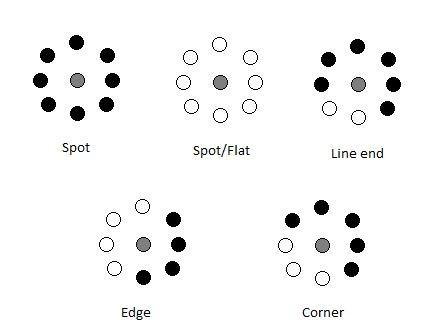
\includegraphics[scale=0.6]{figures/lbp_structural_features} 
\newline
\caption{Patterns that can be detected with uniform LBP}
\label{lbp_structural_features}
\end{center} 
\end{figure}

\phantomsection
\section{Histogram computing}

\vspace{\baselineskip}
\noindent bla
\newline